\documentclass[11pt]{article}
\usepackage[margin=1.1in]{geometry}
\usepackage{amsmath,amssymb}
\usepackage{graphicx}
\usepackage{booktabs}
\usepackage{microtype}
\usepackage[hidelinks]{hyperref}
\usepackage[small,bf]{caption}

\title{Auditing a live packing benchmark:\\
certified GPU refinement and the anatomy of polygon-packing records}
\author{Aristotle Papowitz}
\date{August 2026}

\newcommand{\s}{\ensuremath{s}}

\begin{document}
\maketitle

\begin{abstract}
\noindent
Erich Friedman's Packing Center has curated best-known packings of regular
polygons in regular polygons for more than twenty-five years, and in 2025--26 it
became an arms race: industrial NLP-solver teams, DeepMind's AlphaEvolve, and a
wave of prolific individual contributors now improve its $\sim$490 entries
almost daily. We audit this benchmark with a certified pipeline --- batched
float32 GPU search, on-device float64 refinement, and independent exact
separating-axis certification --- and find that the modern record wave is
systematically under-converged by contributor-specific amounts: entries by two
of the most prolific setters sit $10^{-4}$--$4\times10^{-3}$ above the bottoms
of their own basins, while other contributors, all legacy (1996--2012) entries,
and all closed-form entries are converged to ties. Exploiting this gap and three
structured construction mechanisms, we claimed improved packings for 54 problems
in five days; 52 were credited and 41 still stand six weeks later. Two of the
new records are exact: $160$-digit contact-manifold solving with integer-relation
detection proves 41 and 42 unit squares pack in equilateral triangles of side
exactly $6+8/\sqrt{3}$, and 43 squares in side $5+10/\sqrt{3}$, closed forms
three prior record iterations missed. Negative results delimit what compute
alone can do: random multi-start reproduces known optima up to $n\approx22$ but
cannot reach rearrangement-class basins, locating the frontier in construction,
not optimization. All packings, table snapshots, and a one-command verifier are
public.
\end{abstract}

\section{Introduction}\label{sec:intro}

Since the late 1990s, Erich Friedman's \emph{Packing Center}
\cite{friedman-site,friedman-survey} has maintained tables of the smallest known
regular $M$-gon containing $n$ non-overlapping unit regular $m$-gons ---
24 categories, roughly 490 entries, each attributed to the person who found it.
For most of its history the site was a quiet corner of recreational geometry.
That changed in 2025--26. DeepMind's AlphaEvolve used these tables as a public
testbed for LLM-evolved search programs and took records that still stand
\cite{alphaevolve}; a FICO/ZIB team showed that an off-the-shelf spatial
branch-and-bound stack takes dozens of entries in one sweep
\cite{berthold-oob,berthold-hex}; evolutionary follow-ups beat AlphaEvolve at
its own entries \cite{improvevolve}; and a handful of individuals began
mass-producing records, several hundred between them, with undisclosed
pipelines. During the five days of our campaign the tables moved daily.

This paper treats that moving benchmark as an object of study. We ask three
questions. \emph{How sound are the current records} --- are the listed values
converged, and would they survive independent certification?
\emph{Where do new records actually come from} --- what does each mechanism
(more compute, better refinement, better construction) actually yield? And
\emph{what does it take to claim a record correctly} on a benchmark that moves
under the claimant?

Our instrument is a certified two-phase pipeline (\S\ref{sec:pipeline}):
massively batched float32 search on a consumer GPU, float64 refinement of
survivors, and an \emph{independent} certifier that computes exact
separating-axis margins and a rigorous size bound for every claim. On top of it
we operate four structured mechanisms (\S\ref{sec:mechanisms}): reconstructing
competitors' published images and converging them further; structured
basin-hopping with vacancy and lattice-seeded moves; \emph{drop-one
propagation}, which turns one strong $(n{+}1)$-packing into records at $n$ and
below; and exact contact-manifold solving with PSLQ integer-relation detection,
which here both identifies exact closed forms and certifies their absence.

The audit (\S\ref{sec:results}) produced 54 claimed improvements across 14
tables, of which 52 were credited and 41 still stand at the ledger freeze six
weeks later (Table~\ref{tab:ledger}); every claim in this paper is backed by
public coordinates, a fresh certification run, and archived snapshots of the
tables (\S\ref{sec:repro}). We report the findings a trophy list would hide:
the margin distribution by prior record holder (Fig.~\ref{fig:margins}), which
shows the 2026 wave is under-converged in a contributor-specific way; the
negative results (Table~\ref{tab:negative}), which show random multi-start
stops producing new records around $n\approx22$; and the attrition curve
(Fig.~\ref{fig:attrition}), which quantifies how quickly records on a live
benchmark decay --- two of our claims were invalidated purely by the table
moving between verification and processing.

\section{Records, semantics, and what counts as a claim}\label{sec:semantics}

An entry in category $(m, M)$ at count $n$ is a placement of $n$ unit-side
regular $m$-gons, pairwise non-overlapping, inside a regular $M$-gon of side
$\s$; smaller $\s$ is better. The site displays values truncated to five
decimals with a trailing plus: a listed $\s = x^{+}$ means the incumbent holds
some value in $[x, x+10^{-5})$. Beating an entry therefore requires a
\emph{certified} value strictly below the displayed floor $x$; matching digits
is a tie, and during an active wave the floor itself must be re-read the day of
submission.

We call a packing \emph{certified} when an independent checker --- separate
code from the search --- verifies exact pairwise separation margins (separating
axis over both polygons' edge normals, exact for convex shapes) and exact
containment margins in float64, then converts any residual violation into a
rigorous bound by shrinking the inner polygons and dilating the container. All
54 claims certify with dilation cost at most $10^{-11}$; re-running the
certifier on the exact coordinates we emailed reproduces every claimed value to
$10^{-9}$ (\S\ref{sec:repro}).

Certification is not pedantry; it is where records are won and lost.
Our float32 search stage accepts ``packings'' whose hidden violations reach
$3\times10^{-4}$ --- large enough to fake a record --- and finite-difference
squeezing stalls $\sim2\times10^{-4}$ above true basin bottoms. Both artifacts
produced false records in our own runs before the two-phase discipline was in
place, and \S\ref{sec:results} gives evidence that loose refinement of this
kind, not invalid packings, is the signature failure of the current record
wave.

\section{A certified two-phase pipeline}\label{sec:pipeline}

\paragraph{Search, float32, batched.}
The engine solves many restarts simultaneously as one GPU program (JAX
\cite{jax}): a penalty formulation (squared pairwise overlap plus squared
containment violation) minimized by a natively batched L-BFGS
\cite{lbfgs} --- two-loop recursion and Armijo backtracking vectorized over
instances with per-instance step masks --- inside a shrink-and-anneal outer
loop with kick rescue for stalled instances. A single RTX~4090 sustains
$\approx$127 restarts per minute at $n\approx36$, about $25\times$ a 32-thread
CPU node running the reference implementation \cite{vallejo-packer}, at a total
rented-GPU cost for the campaign of under \$100.
% TODO-V4: pin exact cloud spend from invoices before journal submission.

\paragraph{Refine, float64, on device.}
Each wave's top survivors are promoted to float64 on the GPU and driven through
polish (fixed-size penalty minimization to machine precision), grow-to-feasible,
and squeeze (backtracking container shrink while a machine-precision-valid
packing survives). Only then does the independent certifier of
\S\ref{sec:semantics} run, followed by a same-day re-read of the live table ---
the last gate before any claim is emailed.

\section{Four mechanisms, measured}\label{sec:mechanisms}

\paragraph{1. Reconstruct and squeeze (the audit instrument).}
Record pages publish images, not coordinates. We recover coordinates from a
published GIF/PNG to $\sim$0.1--0.15\,px by fitting shape boundaries subpixel,
then converge the reconstruction in float64. If the incumbent's pipeline was
loose, the same configuration certifies \emph{below their own displayed floor};
if it was tight, we document a tie. This mechanism is simultaneously our audit
probe and our most productive record source: 45 of 54 claims (44 of the 52
credited), with margins up to $3.9\times10^{-3}$ against the quoted entry. It
found closed forms too: reconstructing the freshly-set $n=42$ and $43$
squares-in-triangle entries and squeezing revealed values $4\times10^{-9}$
above $6+8/\sqrt{3}$ and $5+10/\sqrt{3}$ --- staircase-family forms the
incumbent, and two record iterations before him, had approximated numerically
without recognizing (Fig.~\ref{fig:gallery}, center; confirmed exact in
mechanism 4).

\paragraph{2. Structured basin-hopping.}
Random multi-start converges whatever basin it lands in but almost never lands
in a globally rearranged one (\S\ref{sec:results}). Our basin-hopping layer
adds what randomness lacks: an elite pool; vacancy, teleport, shear, and
coherent tilt-cluster moves; and \emph{lattice immigrants} --- exact lattice
packings with deliberate defects injected into the population. Its signature
result is 36 squares in an octagon (Fig.~\ref{fig:gallery}, left). Our first
submission (2.92902\ldots) beat
the listed entry and was accepted --- then superseded within minutes when the
site's maintainer noticed a trivial 37-square diamond lattice at
$10-5\sqrt{2}=2.92893^{+}$ dominating both $n=36$ and $37$ (``you did have the
record, for about 5 minutes''). Re-seeding the search with
\emph{lattice-minus-one} configurations found the vacancy rearrangement at
$\s=2.9287015\ldots$, reclaiming the record over the trivial construction. The
episode is now a checklist item: verify no trivial $(n{+}1)$-construction
dominates before claiming $n$.

\paragraph{3. Drop-one propagation.}
Removing one shape from a strong $(n{+}1)$-packing and re-squeezing all $n{+}1$
removal variants costs one batched GPU call, and when the $(n{+}1)$ basin has
better architecture than the incumbent at $n$, the improvement cascades
downward. From our own 35 triangles-in-octagon basin this produced $n=34$ at
$1.86454^{+}$ (Fig.~\ref{fig:gallery}, right; $7.2\times10^{-3}$ below our
week-old value) and then $n=33$ at
$1.84789^{+}$, halting at $n=32$ where the incumbent architecture is already
strong. Measured yield across $\sim$400 seed packings: exactly one such
cascade --- rare, but each hit is worth multiple records, and the mechanism
explains the observed monotonicity anomalies on the site (at this writing the
triangles-in-pentagon table still lists $n=44$ at $3.52140^{+}$, \emph{worse}
than $n=45$ at $3.51261^{+}$, an inconsistency drop-one would repair if the
$n=45$ coordinates were public).

\paragraph{4. Exact contact solving and PSLQ.}
For converged packings we extract the active contact graph (vertex--edge,
vertex--wall), select independent constraints by pivoted QR, and solve the
contact-manifold KKT system by minimum-norm Gauss--Newton in 160-digit
arithmetic \cite{mpmath}; convergence is quadratic ($|F|:10^{-8}\!\to\!10^{-160}$
in five iterations) even on floppy manifolds. PSLQ \cite{pslq} then hunts
integer relations on the refined $\s$. Both outcomes occur, and both matter:

\emph{Identification.} The squares-in-triangle configurations at $n=41,42$
solve to the exact root of $3\s^{2}-36\s+44$, i.e.\
$\s=6+8/\sqrt{3}=10.6188021535\ldots$, and $n=43$ to the root of
$3\s^{2}-30\s-25$, i.e.\ $\s=5+10/\sqrt{3}=10.7735026918\ldots$, matching the
algebraic forms to all 65 computed digits. Our submitted float64 records sit
$3.7\times10^{-9}$ and $7.0\times10^{-9}$ above the exact bottoms (identical
truncated display). Contact structure: at $n=43$ only 25 of 43 squares are
load-bearing, on a 13-dimensional floppy manifold.

\emph{Refutation.} For 26 squares in an octagon (our record $2.52709\ldots$),
the same pipeline certifies at 65 digits that \emph{no} minimal polynomial of
degree $\le 8$ with coefficients up to $10^{8}$ exists, and no relation in
$\mathbb{Q}(\sqrt{2+\sqrt{2}})$ despite the packing's $22.5^{\circ}$ tilt
structure --- a no-closed-form certificate (4 rattlers, 8 floppy modes, 59
independent contacts). The same computation acts as a super-polisher, locating
basin bottoms a few $10^{-9}$ below float64 values.

\begin{figure}[t]
\centering
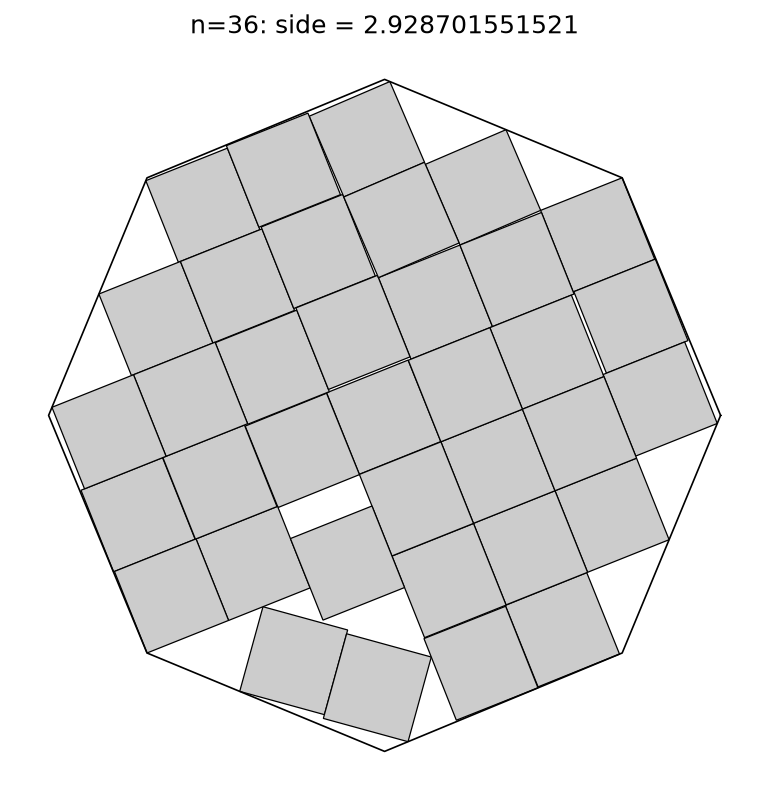
\includegraphics[height=1.58in]{figures/gallery_squoct36}\hfill
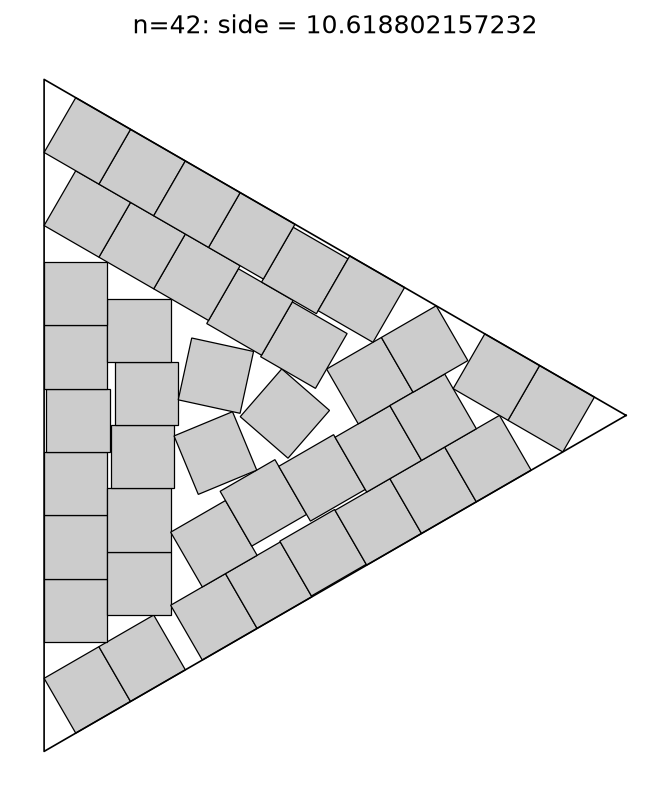
\includegraphics[height=1.58in]{figures/gallery_squtri42}\hfill
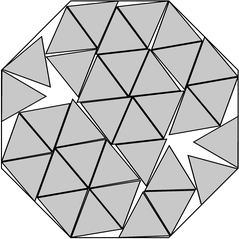
\includegraphics[height=1.58in]{figures/gallery_trioct34}
\caption{Flagship records of three mechanisms. \emph{Left}: 36 squares in an
octagon of side $2.92870^{+}$ --- a vacancy rearrangement of the trivial
37-square diamond lattice, found by basin-hopping seeded with lattice-minus-one
configurations. \emph{Center}: 42 squares in an equilateral triangle of side
exactly $6+8/\sqrt{3}$, recovered from the incumbent's published image and
squeezed onto the closed form (proved exact in \S\ref{sec:mechanisms}).
\emph{Right}: 34 triangles in an octagon of side $1.86454^{+}$, obtained by
deleting one triangle from a stronger 35-triangle packing and re-squeezing.}
\label{fig:gallery}
\end{figure}

\section{The audit}\label{sec:results}

\begin{table}[t]
\centering\small
\caption{The campaign ledger, summarized per table (freeze 2026-08-16).
``Credited'' means the credit is verified in an archived snapshot of the live
table; margins are lower bounds against the displayed floor of the entry
beaten. The per-problem ledger with full-precision values, mechanisms, and
per-claim status is in the repository (\texttt{LEDGER.md}).}
\label{tab:ledger}
\begin{tabular}{lccccc}
\toprule
Table & $n$ range & Claimed & Credited & Standing & Margin range \\
\midrule
Squares in octagons     & 26--40 & 9 & 9 & 4 & $1.5\times10^{-5}$--$3.9\times10^{-3}$ \\
Triangles in pentagons  & 28--43 & 8 & 8 & 8 & $5.8\times10^{-5}$--$3.3\times10^{-3}$ \\
Pentagons in hexagons   & 6--31  & 7 & 6 & 4 & $9.3\times10^{-5}$--$3.2\times10^{-3}$ \\
Triangles in octagons   & 31--37 & 7 & 7 & 7 & $3.0\times10^{-5}$--$7.4\times10^{-3}$ \\
Hexagons in pentagons   & 5--32  & 5 & 5 & 4 & $1.6\times10^{-6}$--$1.6\times10^{-3}$ \\
Pentagons in octagons   & 28--31 & 4 & 3 & 1 & $2.4\times10^{-4}$--$1.1\times10^{-3}$ \\
Squares in triangles    & 41--43 & 3 & 3 & 3 & $4.3\times10^{-4}$--$7.6\times10^{-4}$ \\
Hexagons in hexagons    & 32--33 & 2 & 2 & 2 & $1.3\times10^{-4}$--$7.6\times10^{-4}$ \\
Octagons in hexagons    & 6, 20  & 2 & 2 & 1 & $1.5\times10^{-4}$--$2.3\times10^{-3}$ \\
Octagons in triangles   & 14, 18 & 2 & 2 & 2 & $8.5\times10^{-4}$--$1.6\times10^{-3}$ \\
Squares in hexagons     & 30, 40 & 2 & 2 & 2 & $1.1\times10^{-5}$--$1.6\times10^{-5}$ \\
Pentagons in squares    & 8      & 1 & 1 & 1 & $3.9\times10^{-7}$ \\
Pentagons in triangles  & 26     & 1 & 1 & 1 & $7.4\times10^{-4}$ \\
Triangles in hexagons   & 36     & 1 & 1 & 1 & $1.2\times10^{-5}$ \\
\midrule
Total & & 54 & 52 & 41 & $3.9\times10^{-7}$--$7.4\times10^{-3}$ \\
\bottomrule
\end{tabular}
\end{table}

\paragraph{Scale and outcome.}
In five days (July 4--8, 2026) the pipeline produced certified improvements for
54 problems across 14 of the 24 tables (Table~\ref{tab:ledger}). Fifty-two were
credited on the live site; at the ledger freeze on August 16, 41 still stand.
The two uncredited claims fell to the benchmark itself, not to invalid
packings: one was overtaken by a competitor's better value posted the day the
batch went out, and one targeted a floor that was stale by the time of
processing --- we do not count either. Every one of the 54 packings, plus a
certified tie used to validate the submission channel, re-certifies today from
the exact coordinates submitted.

\begin{figure}[t]
\centering
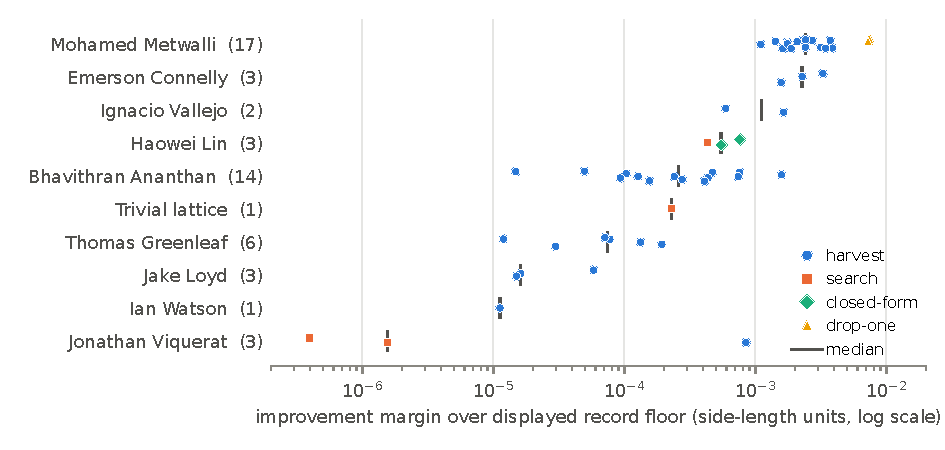
\includegraphics[width=\textwidth]{figures/fig_margins}
\caption{Improvement margin versus prior record holder for 53 claims (log
scale; the stale-floor claim is excluded). Vertical bars mark per-holder
medians; marker shape and color give the mechanism. The 2026 mass-production
wave is under-converged by contributor-specific amounts --- entries we took
from the two most prolific setters sit $10^{-4}$--$4\times10^{-3}$ above their
own basins' bottoms --- while other contributors' entries yield only at the
$10^{-5}$--$10^{-6}$ scale, if at all. The margin is a lower bound on the
incumbent's convergence gap.}
\label{fig:margins}
\end{figure}

\paragraph{Convergence demographics.}
Figure~\ref{fig:margins} plots each claim's margin against the prior holder of
the entry. The pattern is stark and contributor-specific. Entries taken from
the two most prolific 2026 setters cluster at margins of $10^{-4}$ to
$4\times10^{-3}$: their pipelines produce genuinely new configurations whose
final refinement stops three to four decimals short of the basin bottom.
Entries by other active contributors yielded only at the $10^{-5}$ scale or
below --- three fell only to exhaustive search at the sixth decimal
($3.9\times10^{-7}$ in the extreme case) --- and an entire further class never
yielded at all: every legacy entry we attacked (1996--2012, including four
triangles-in-hexagon basins re-converged to nine digits) and every closed-form
entry proved to be an exact tie. The benchmark's weakness is thus not wrong
packings but \emph{loose refinement at scale}, invisible under five-decimal
truncation until someone re-converges the published images.

\begin{table}[t]
\centering\small
\caption{Negative results. Each row is a documented dead end; together they
locate the open frontier in construction rather than compute.}
\label{tab:negative}
\begin{tabular}{p{0.42\textwidth}p{0.52\textwidth}}
\toprule
Experiment & Outcome \\
\midrule
$n=9$--$12$, all 24 tables (69 entries searched) & Zero improvements; the band
is fully converged by the 2025--26 wave, including AlphaEvolve's
hexagons-in-hexagons $n=12$, which our searches tie but do not beat. \\
Legacy entries, e.g.\ triangles-in-hexagons $n=8,16,17,18$ (2005--2012) &
Reproduced to $10^{-9}$: exact ties. Legacy $\ne$ soft. \\
Triangles-in-hexagons $n=21$ control (a better basin is \emph{known} to exist)
& Never found: 4,700+ independent starts plus 400+ structured basin-hopping
rounds converge to $1.99877$, above the known $1.99869^{+}$ --- random
multi-start cannot reach rearrangement-class basins. \\
Trivial plateaus (e.g.\ $\s=2$ at $n=22$--$24$ triangles-in-hexagons;
$4+4\sqrt{2}$ octagons-in-squares) & Rigid under every move class tried;
float32 ``sub-plateau'' sightings were violations in disguise. \\
Drop-one sweep over $\sim$400 seed packings & One cascade
(\S\ref{sec:mechanisms}); all other neighbors tight. \\
\bottomrule
\end{tabular}
\end{table}

\paragraph{Where compute stops.}
Table~\ref{tab:negative} summarizes the campaign's dead ends. The pipeline
reproduces known optima essentially everywhere it lands ($n\lesssim22$), and at
the one control point where a better basin is known to exist ---
triangles-in-hexagons $n=21$ --- thousands of independent starts never find it.
On fresh large-$n$ tails the gap is structural, not numerical: at $n=28$
triangles-in-hexagons our best wave landed $1.1\times10^{-2}$ above the
incumbent, a different architecture altogether. The conclusion, consistent
with the methods used by the currently successful setters
\cite{alphaevolve,berthold-oob,improvevolve}, is that further progress is
construction-limited: the payoff is in seeded, structured moves --- lattice
defects, warm-started global solves, evolved move programs --- not in more
restarts. Consistent with this, one published ablation reports symmetry
\emph{constraints} making 539 of 750 instances worse \cite{berthold-oob};
seeding with symmetric configurations, by contrast, is what won our $n=36$.

\begin{figure}[t]
\centering
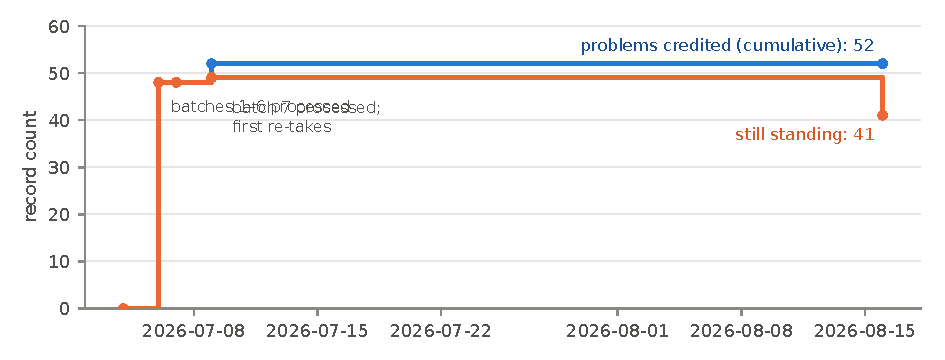
\includegraphics[width=\textwidth]{figures/fig_attrition}
\caption{Benchmark velocity. Cumulative credited problems (blue) versus still
standing (orange) across our archived snapshots. Eleven credits were re-taken
within six weeks by four competitors; two further claims (not shown) were
invalidated before processing by the table moving. Record claims on a live
benchmark are date-stamped statements, not permanent facts.}
\label{fig:attrition}
\end{figure}

\paragraph{Benchmark velocity.}
Figure~\ref{fig:attrition} shows the fate of the 52 credits. Within six weeks,
eleven were re-taken by four competitors; earlier, four \emph{finished} records
were beaten by a competitor while they sat staged for thirty hours awaiting
submission, and were never sent. This velocity has methodological consequences
we adopted and recommend: verify against the live table the day of submission;
archive dated snapshots (ours are in the repository and back every status in
Table~\ref{tab:ledger}); and treat every claim as date-stamped. It also has a
scientific one: a benchmark whose entries change daily but whose history is not
archived anywhere silently loses the provenance of its own frontier.

\section{Discussion}\label{sec:discussion}

Three lessons generalize beyond this benchmark. First, \emph{certification is
cheap and decisive}: exact-margin verification plus a rigorous dilation bound
costs milliseconds per packing, would have prevented every false record we
generated internally, and --- applied by a third party --- revealed that a large
fraction of a 490-entry benchmark sits measurably above its own basins' bottoms.
Live optimization benchmarks (packing sites, but equally leaderboards for
heuristics) would benefit from requiring machine-checkable certificates and
full-precision coordinates rather than images. Second, \emph{refinement and
construction are different resources}. GPU-scale refinement harvested 45
records here, but it is a one-time dividend: once the loose entries are gone
(several competitors re-converged their own entries within days of our wave),
what remains is the construction problem, where our thousands of restarts
bought nothing that structure did not. Third, \emph{exact solving belongs in
the loop}: feeding converged numerical packings to arbitrary-precision contact
solving identified three records as exact algebraic values ($6+8/\sqrt{3}$
twice, $5+10/\sqrt{3}$) and certified a fourth as having no simple closed form,
at negligible cost next to the search that found them.

Limitations: all values are upper bounds --- nothing here is proved optimal, in
contrast to interval-arithmetic work on circle packings \cite{markot-csendes};
the audit covers one benchmark family (regular polygons in regular
containers); and our exact-form statements certify the contact system of our
configurations, not global optimality at those $n$.

\section{Reproducibility and disclosure}\label{sec:repro}

The toolkit, the per-problem ledger, all 54 coordinate sets (plus the
validation tie), the certification table, and dated scrapes of all 24 record
tables are public at
\url{https://github.com/AriPapowitz/polygon-packing-records}. One command
re-certifies every claim from the submitted coordinates
(\texttt{paper/collect\_and\_certify.py}); the ledger and figures regenerate
from the archived snapshots. The engine extends an open-source packer
\cite{vallejo-packer} (GPL-3.0) with the batched GPU search, float64
refinement, certification, reconstruction, and exact-solving layers.

This campaign was conducted with substantial AI assistance (Claude, Anthropic):
the code was largely AI-written under the author's direction, and overnight
search campaigns ran autonomously. Every packing is machine-generated,
independently certified by the tooling described here, and was verified by the
site's maintainer before listing. % Disclosure per venue policy; expand as required.

\paragraph{Acknowledgments.}
Erich Friedman has maintained the Packing Center, and processed a great many
submissions including ours, with patience and care. The competitors whose
entries seeded our harvests --- and who re-took eleven of them within weeks ---
made the benchmark the live, adversarial object this paper studies.

\begin{thebibliography}{19}\small

\bibitem{friedman-site} E.~Friedman. \emph{Erich's Packing Center}.
\url{https://erich-friedman.github.io/packing/}. Accessed 2026-08-16; dated
snapshots archived in the repository.

\bibitem{friedman-survey} E.~Friedman. Packing unit squares in squares: a
survey and new results. \emph{Electron.\ J.\ Combin.}, Dynamic Survey DS7.

\bibitem{alphaevolve} A.~Novikov et al. AlphaEvolve: a coding agent for
scientific and algorithmic discovery. arXiv:2506.13131 (2025).
% TODO-V5: confirm author list.

\bibitem{berthold-oob} T.~Berthold et al. Out-of-the-box global optimization
for packing problems. arXiv:2605.04850 (2026). % TODO-V5: confirm title/authors.

\bibitem{berthold-hex} T.~Berthold et al. Packing regular hexagons with
NLP solvers. arXiv:2601.05943 (2026). % TODO-V5: confirm title/authors.

\bibitem{improvevolve} ImprovEvolve: seeded LLM-evolved basin hopping for
packing. arXiv:2602.10233 (2026). % TODO-V5: confirm title/authors.

\bibitem{vallejo-packer} I.~Vallejo (``Flamethr0wer''). \emph{polygon-packer}.
\url{https://github.com/Flamethr0wer/polygon-packer}.

\bibitem{gensane} T.~Gensane and P.~Ryckelynck. Improved dense packings of
congruent squares in a square. \emph{Discrete Comput.\ Geom.}\ 34 (2005)
97--109.

\bibitem{markot-csendes} M.~C.~Mark\'ot and T.~Csendes. A new verified
optimization technique for the ``packing circles in a unit square'' problems.
\emph{SIAM J.\ Optim.}\ 16 (2005) 193--219.

\bibitem{nurmela} K.~J.~Nurmela and P.~R.~J.~\"Osterg\aa rd. Packing up to 50
equal circles in a square. \emph{Discrete Comput.\ Geom.}\ 18 (1997) 111--120.

\bibitem{graham-lubachevsky} B.~D.~Lubachevsky and R.~L.~Graham. Dense packings
of congruent circles in a circle. \emph{Discrete Math.}\ 181 (1998) 139--154;
see also arXiv:math/0405310, arXiv:math/0406252.

\bibitem{specht} P.~G.~Szab\'o and E.~Specht. Packing up to 200 equal circles
in a square. In \emph{Models and Algorithms for Global Optimization}, Springer
(2007); packings at \url{http://www.packomania.com}.
% TODO-V5: confirm exact chapter reference.

\bibitem{amore} P.~Amore. Circle packing in regular polygons.
arXiv:2212.12287 (2022). % TODO-V5: confirm title.

\bibitem{kampas} F.~J.~Kampas, J.~D.~Pint\'er, and I.~Castillo. Packing ovals
in optimized regular polygons. arXiv:1901.07056 (2019). % TODO-V5: confirm.

\bibitem{viquerat-pbo} J.~Viquerat et al. Policy-based optimization:
single-step policy gradient method seen as an evolution strategy.
arXiv:2104.06175 (2021).

\bibitem{pslq} H.~R.~P.~Ferguson, D.~H.~Bailey, and S.~Arno. Analysis of PSLQ,
an integer relation finding algorithm. \emph{Math.\ Comp.}\ 68 (1999) 351--369.

\bibitem{mpmath} F.~Johansson et al. \emph{mpmath: a Python library for
arbitrary-precision floating-point arithmetic}, version 1.3.

\bibitem{jax} J.~Bradbury et al. \emph{JAX: composable transformations of
Python+NumPy programs}, 2018. \url{http://github.com/google/jax}.

\bibitem{lbfgs} D.~C.~Liu and J.~Nocedal. On the limited memory BFGS method
for large scale optimization. \emph{Math.\ Program.}\ 45 (1989) 503--528.

\end{thebibliography}

\end{document}
